\documentclass{article}
\usepackage[utf8]{inputenc}
\usepackage{amsmath}
\usepackage{amsfonts}
\usepackage{tikz}
\usepackage{tkz-euclide}

\begin{document}

\begin{center}
    \section*{Maths Problems Set 2 (24 December 2019)}
\end{center}

\begin{enumerate}
    \item
    The vertices of a square are labelled $A$, $B$, $C$ and $D$ going anticlockwise, and a random point $P$ in the square is chosen. What is the probability that angle $\angle{APB}$ is obtuse?
    
    \item
    Two particles are travelling in opposite directions with the same speed. After the collision they travel in the same direction. What can be said about their relative masses?
    
    \item
    How many trailing zeroes does 100! have?
    
    The number of trailing zeroes a natural number has is the number of zeroes after the last non-zero digit. For example, 2\textbf{00} has 2 trailing zeroes, 130452\textbf{0} has 1 trailing zero, and 14 has no trailing zeroes.
    
    $n! = n \times (n - 1) \times (n - 2) \times ... \times 3 \times 2 \times 1$, so $100! = 100 \times 99 \times 98 \times ... \times 3 \times 2 \times 1$.
    
    \item
    
    Find the area of the square in the diagram below, given that the radius of each of the circles is 1.
    
    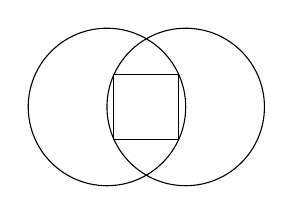
\begin{tikzpicture}[scale=0.5]
        \draw (-1, 0) circle [radius=2];
        \draw (1, 0) circle [radius=2];
        \draw ({sqrt(2-(sqrt(7)/2))}, {sqrt(2-(sqrt(7)/2))}) -- ({sqrt(2-(sqrt(7)/2))}, {-sqrt(2-(sqrt(7)/2))}) -- ({-sqrt(2-(sqrt(7)/2))}, {-sqrt(2-(sqrt(7)/2))}) -- ({-sqrt(2-(sqrt(7)/2))}, {sqrt(2-(sqrt(7)/2))}) -- cycle;
    \end{tikzpicture}
    
    \item
    In the Gregorian calendar where dates are denoted in the form dd/mm/yyyy, how many dates are there between 1 January 1900 and 31 December 1999, inclusive, where the date contains no repeated digits?
    
    \item
    Timmy pulls a crate with a mass of 10 kg along a flat surface with a constant force of 200 N. The crate is pulled at a angle so as to maximise its acceleration. The coefficient of friction between the crate and ground is $\frac{1}{\sqrt{2}}$. Timmy eventually releases the crate allowing friction to bring it to rest. Given that the journey took 40 seconds, how far did the crate travel?
    
    \item
    Two players are playing a game wherein they take turns subtracting from a positive integer running total (starting from $T$). Each player may only subtract a power of 2 from the total each turn. The player who reduces the running total $T$ to 0 wins. For what $T<100$ would you want your opponent to take the first move?
    
    The game is then changed so that instead of subtracting powers of 2, each player can subtract any number from the set $A$, where $A$ is a proper subset of the natural numbers. Show that there always exists a value for $T$ such that you want your opponent to take the first move.
    
    \item
    Find an expression for $\int_0^n \lfloor 2^x \rfloor \text{ } \mathrm{d}x$ where $n$ is a positive integer.
    
    \item
    A University bike shed contains $n$ cubicles in a row. Each cubicle stores one bicycle. 
    
    One morning, Professor Ponte places his bicycle in one of the cubicles. At night Priyanka attempts to steal his bike by opening one and only one of the cubicles. The next morning Professor Ponte moves his bike from the cubicle it is currently in to one of the cubicles adjacent to the one it was in before, and closes the cubicle that Priyanka opened. Note that if the bicycle is in one of the cubicles at the end then there is only one possible cubicle for it to be moved to the follow morning. This repeats every morning and corresponding night.
    
    Devise a general strategy for Priyanka to successfully steal Professor Ponte's bike. Note that your strategy must work for any number $n$ of cubicles in the bike shed.
    
    \item
    There is a pile of 129 coins on a table, all unbiased except for one which has heads on both sides. Bob chooses a coin at random and tosses it eight times. The coin comes up heads every time. What is the probability that it will come up heads the ninth time as well?
    
    \item
    The sum $S_n$ is defined by $S_n = \sum\limits_{k=1}^{n} n(2^n)$, i.e. $2 + 8 + 24 + ... + n(2^n)$.
    
    Find an expression for $\sum\limits_{k=1}^n S_k$, i.e. $S_1 + S_2 + S_3 + ... + S_n$.
    
    \item
    It is tradition for gnomes to give gifts in a very peculiar manner. First all the gnomes stand in a circle. Starting with the longest bearded gnome a gift is given to the next standing gnome in the circle. That gnome then sits down to open their present and the process repeats from the next gnome standing. Given that there are $n$ gnomes in the circle, at what position in the circle is the last standing gnome who therefore doesn’t get a gift?
    
    \item
    Let $a$ and $b$ be positive integers. Show that $\sqrt{2}$ always lies between $\frac{a}{b}$ and $\frac{a+2b}{a+b}$, inclusive.
    
    \item
    Consider the numbers 1, 2, ..., n. Find, in terms of n, the largest integer t such that these numbers can be arranged in a row so that all consecutive terms differ by at least t.
    
    \item
    A piece on a infinite chess board can move $A$ spaces along one of the axes and $B$ spaces along the other in a single move (like a bizarre knight). For what values of $A$ and $B$ can the knight reach any given square on the board?
    
    \item
    Given a triangle with side lengths 41, 39 and 50, find the radius of the circumscribed circle.
    
    
    
    
\end{enumerate}



\end{document}
